%%!TEX root=../main.tex


\section{METHODOLOGY}
\subsection{Setting Scenario}
The goal of this paper is to find the location of the tennis ball. 
Thus, the first step is to set the sensors. According to the symmetric, except the area of the net, the other parts of the tennis court could be treated as the same situation. In order to prevent the settled sensors from affecting the athletes, our plan is to set up sensors around the tennis court so that the transmission range of sensor signals can surround the whole court. As shown in the figure \ref{sensors}, take the 2 meters left of the intersection point of the bottom line and the left doubles sideline as the coordinate origin, and establish the coordinate system. In addition, we considered that place a tiny chip in tennis which could send a signal when the ball drop on the grand.\\
\begin{figure}[ht]
\centering
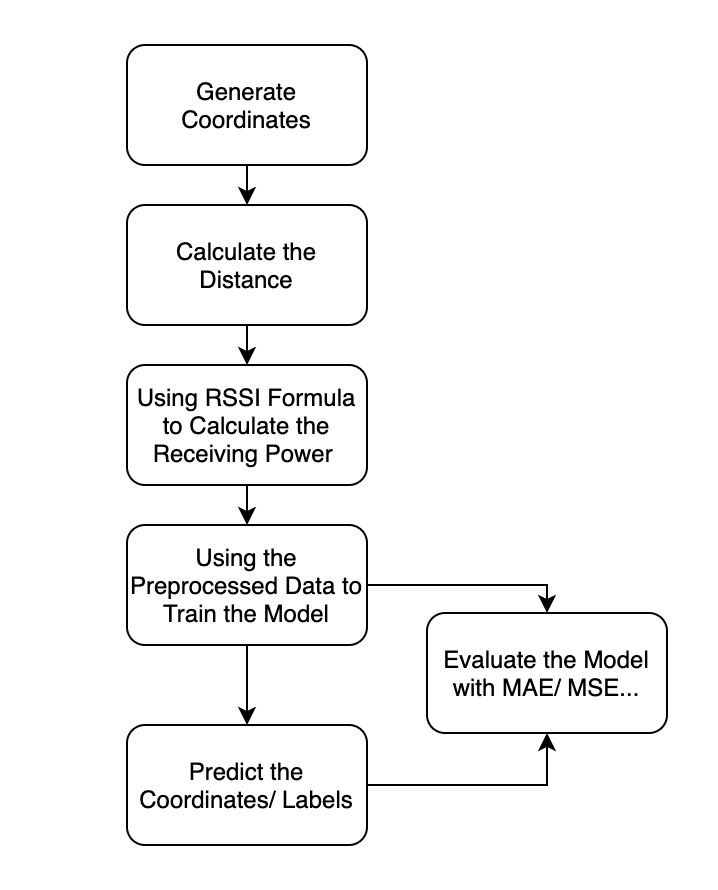
\includegraphics[width=3in]{\FIGDIR/P7_Flow.png}
\caption{The Flow Chart of Simulation}
\label{flow chart}
\end{figure}

\begin{figure}[ht]
\centering
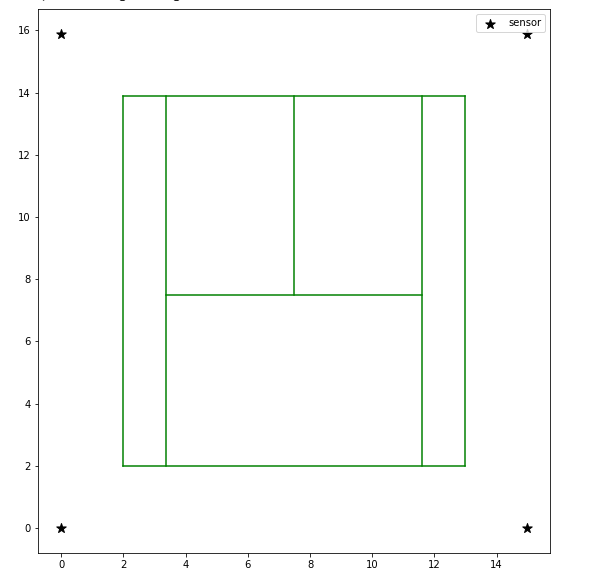
\includegraphics[width=3in]{\FIGDIR/P6_SetSensor.png}
\caption{The Schematic Diagram of Setting Sensors}
\label{sensors}
\end{figure}
\subsection{Choosing Localization algorithm}
We further assume the relationship between a tennis ball and the settled sensors are a relatively static state. Then the method for localization could be narrow down into static landmarks with static nodes. The category of static landmarks with static nodes including range-free and range-based. As mentioned above, the range-based approaches are more proper for our scenario. Considering that the service speed of the tennis ball can reach more than 200km/h, we believe that the time-based measurement method cannot capture such a fast ball. In addition, in wireless sensor network, it is very difficult to synchronize the time of sensors, which increases the error and reduces the accuracy to some extent. Therefore, from the ToA, TDoA, AoA and RSSI methods, we chose the RSSI as our localization algorithms based on the requirements of precision and accuracy.\\

\subsection{LSTM based Model}
The flow chart of the simulation is shown in the figure \ref{flow chart}. The first step is to create the dataset. Because the LSTM model has the memory of the previous information, based on the different techniques of each player, in order not to increase redundant information, we just use one match as a unit. On the professional circuit, men play best-of-five-set matches at the Grand Slam tournaments, we assuming that for one match: each set has 12 games, each game has 8 points (just one deuce included), each point has one batting with one double fault serve, and we could have our upper bound of the positions: overall 1440 drop points of balls. With the same principle, except the men's singles of the Grand Slam tournaments, others are best-of-three-set matches. Suppose for one match: without any double fault for service as well, each set has 6 games, each game has 4 points, we will have 216 drop points of balls. Therefore, the upper bound for our dataset is 1440 and lower bound is 216. Considering that the number of Masters tournaments are much greater than the Grand Slam tournaments, we first used 500 as our dataset size.

We randomly generate 500 two-dimensional coordinates in the established Cartesian coordinate system. These coordinates are used for labels for training the model. And the coordinates are further used with the Euclidean distance formula to calculate the distance between the ball to the sensors.\\
\begin{equation}
    D = \sqrt{(y_2-y_1)^2+(x_2-x_1)^2}
\end{equation}

As mentioned above, the RSSI could be calculated by the equation (6), which is the sum of the transmitting power, the gain of transmitting, the gain of receiving and free-space transmission loss. The transmitting power is fixed value which we assume is 10 dBm. If we chose the fixed double plate directional antenna the range of transmitting could cover at least half of the tennis court. The working frequency of such antenna is from the 2400 MHz to 2525 MHz and the gain of receiving normally is 14 dB. The free-space transmission loss could be calculated by the equation (7). The formula (7) is a generic form of free-space transmission loss in the metric system of units. Since in actual links, the frequency is in MHz or GHz and distance in km, by using $c = 3 \times 10^8$ m/s, then free-space transmission loss is specified by one of the following formula:\\
\begin{equation}
    L_p = 32.4 + 20 log f + 20 log d
\end{equation}

And if the sensors are working in the 25 centigrade and 1 atmosphere, we could think the transmission power is 2400 MHz. If the sensors are working in the 25 centigrade and 1 atmosphere, we could think the transmission power is 2400 MHz. Therefore, by using the formula (18), we could transfer the distances of dataset into receiving power which is the input of the model. And by setting the random state as 42, 80\% data are taken out as train set.

Before using the created data to feed our model, the data need to preprocess. The method we chose is standardization. As shown in equation (19), the standardization is to scale proportionally and falls into a small interval. To be more specific, standardizing a vector means subtracting a measure of location and dividing it by a measure of scale. After standardization, all attributes of data will have the same weight.\\ 
\begin{equation}
    x^*=\frac{x-\mu}{\sigma}
\end{equation}

The structure of the model \cite{tarwani2017survey} is shown in the figure \ref{LSTM structure}. It consists of two LSTM layers and a fully-connected layer. The first LSTM layer fed the data of the training set and returns all hidden states obtained according to the input to the next LSTM layer. Since the required output is the two-dimensional coordinates of the placement, the number of neurons in the fully-connected layer is set to 2. 

\begin{figure}[ht]
\centering
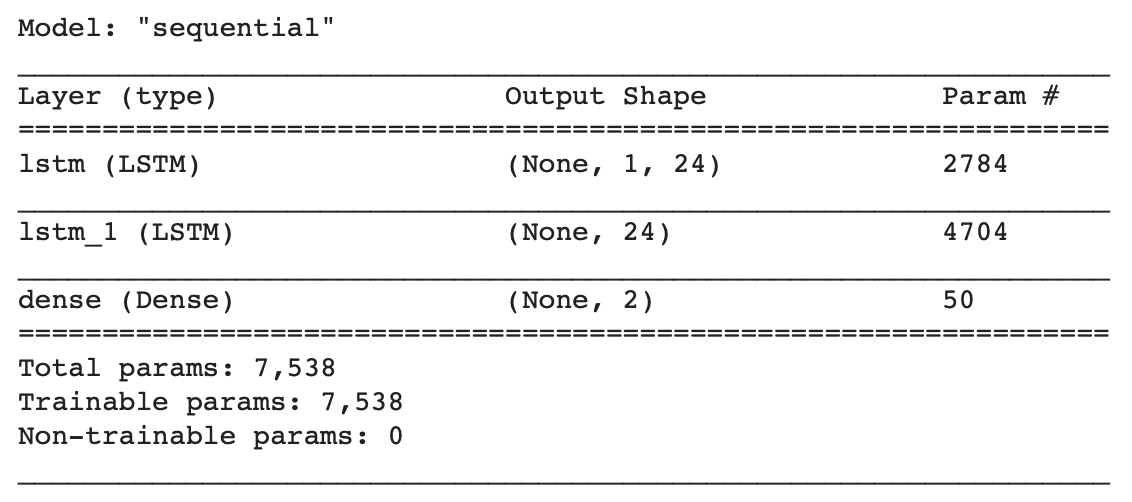
\includegraphics[width=3in]{\FIGDIR/P8_LstmModel.png}
\caption{The LSTM Model}
\label{LSTM structure}
\end{figure}
During the compilation of the model, in order to make the model converge, we set the number of epochs as 2000. When the entire dataset passes through the neural network once and returns once, this process is called an epoch. If the number of epochs is too small, the model will be underfitting, which will not reach the expected accuracy. If too many epochs were set, the model would overfit and would not perform well in the test set.

The batch size as 10. If the batch size is too small, the training data will be difficult to converge, resulting in underfitting. Since we have a total of 500 samples and the batch size is 10, 50 iterations are needed to train the complete sample set.

For the training set, we extract 20\% as the validation set and set validation frequency to 1. The validation set is used to test the state and convergence of the model in the training process. At the same time, the validation set can also be used to monitor whether the model has been overfitted. Generally speaking, after the verification set is stable, if the training continues, the performance of the training set will continue to rise, but the validation set will not rise but fall, so the overfitting generally occurs. So the validation set is also used to determine when to stop training.

The initial learning rate was set to 0.001, and when the model stopped being promoted, the ReduceLROnPlateau function was set as a monitor. The patience is set as 3 which means if 3 epochs with no improvement after which the learning rate will be reduced. The learning rate will be reduced following the equation: 
\begin{equation}
lr_{new} = lr \times factor    
\end{equation}
Where the factor is 3. And the minimum learning rate is set as 0.00001 in case of the learning rate is too small.

In addition, we used Adam \cite{kingma2014adam} as the optimizer to adjust the weights of the model.The Adam algorithm considers the first-moment estimation (the mean value of the gradient) and the second-moment estimation (the non-centralized variance of the gradient) to calculate the update step size.


\subsection{MLP based model}
In the last section, we used RSSI as input to predict the tennis ball's placement point. With these coordinates, we can help athletes better analyze their own or opponent's technical characteristics, so as to improve their skills or change strategies. However, in the tennis match, we are more concerned about whether tennis is out of bounds, so we can use the MLP model to simplify the problem to the classification problems.

The processing of the data is basically the same as in the previous section: 500 coordinates are generated randomly, the distance between the coordinates and the sensor is calculated, and then the received power is calculated according to the RSSI formula. However, the labels of the dataset need to judge the distance between the coordinate and the sensor according to the size of the tennis court. If the coordinate out of the boundary, that is, the coordinates beyond the range of size of the tennis court are marked as 0. Also, mark the coordinates that are not out of bounds as 1. Establish the label of the data set in the above method.

The MLP model structure is shown in the figure \ref{MLP structure}. The model is composed of three fully-connected layers and two dropout layers. The number of neurons in the first two fully-connected layers is 32. In the last fully-connected layer, only one neuron is needed because only one value is output for the classification problem. The purpose of the dropout layer is to discard some neural network units from the network according to a certain probability during the training process, which is equivalent to finding a more concise network from the original network. Our ratio is set at 0.2, which means that 0.2 of neurons will be discarded from the MLP network through the dropout layer. Setting the dropout layer can prevent the model from overfitting and save training time.

\begin{figure}[ht]
\centering
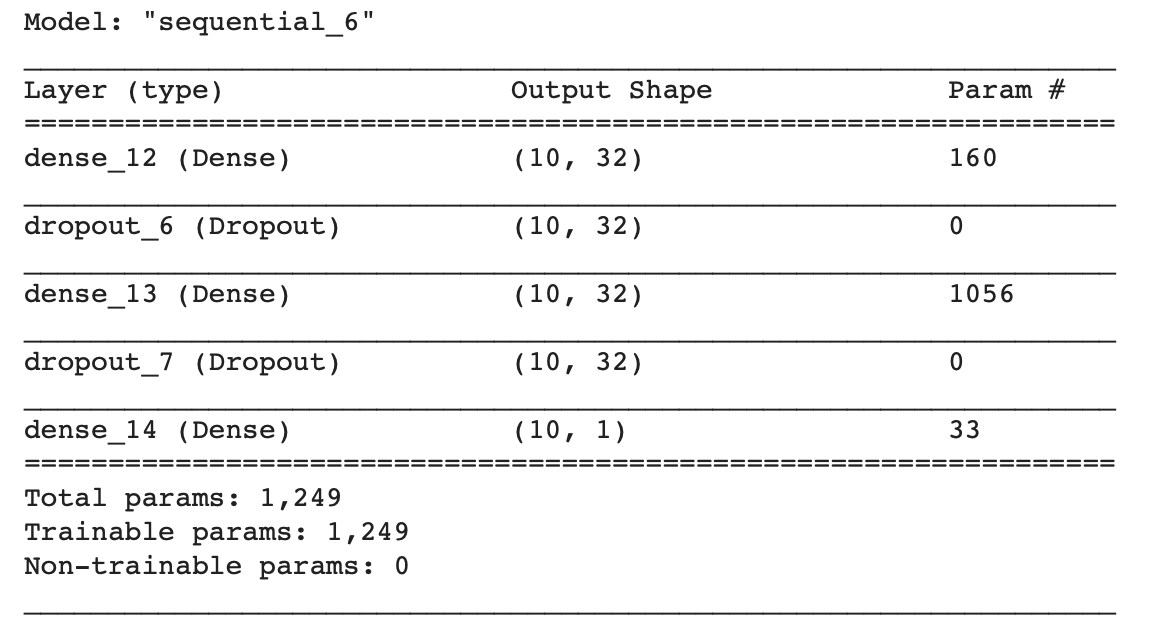
\includegraphics[width=3in]{\FIGDIR/P13_MlpModel.png}
\caption{The MLP Model}
\label{MLP structure}
\end{figure}
The number of the epoch is set to 800. We tried to adjust this number, but the accuracy of the 800 epoch is the highest. Like the LSTM model, the batch size is set to 10, 20\% of the training set is used as the validation set, the validation frequency is 1, and the ReduceLROnPlateau function is set to monitor the training. Unlike the LSTM model, the loss function used to validate the model is binary\_crossentropy instead of the original MAE.  The expression of the binary\_crossentropy function is:
\begin{equation}
    loss = - \sum_{i=1}^n y_i log \hat{y}_i + (1 - y_i ) log(1 - \hat{y}_i)
\end{equation}
The binary\_crossentropy is for the loss function between probabilities, and the loss is zero only if $y_i$ is equal to $\hat{y}_i$, otherwise, the loss is a positive number. Moreover, the greater the difference in probability, the greater the loss. 
\subsection{SVM-based model}
As mentioned in last section, we could use SVM, a non neuron network model, to classify the data. For SVM there are some parameters we have to set. One of the most import parameter is the C value also named regularization parameter. The larger the C is, the smaller the margin is, conversely, if the C-value is small, the margin will be big, which means there will be more data-points could be misclassified by the model. To find a best C, first we set a random list and to observe the tendency of the curve. Then we change the range of the list which will near the best parameter obtained by last trying, Therefore, from figure \ref{SVM1} and \ref{SVM2}, we got 18 as the best value for C. Besides parameter C, we use RBF as our kernel function which map our data to high dimension which let them be linearly separable and use scale as the gamma of the kernel function. 
\begin{figure}[ht]
\centering
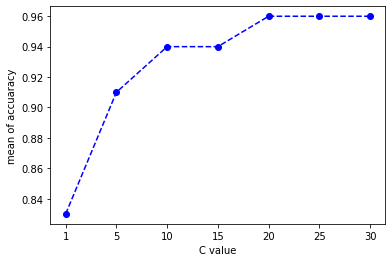
\includegraphics[width=3in]{\FIGDIR/svm1.png}
\caption{The Mean of Accuracy with Different C Values}
\label{SVM1}
\end{figure}
\begin{figure}[ht]
\centering
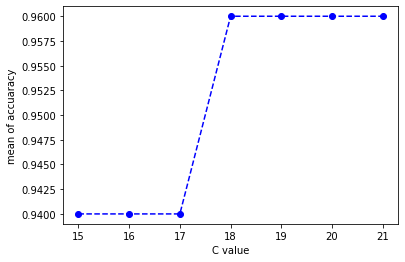
\includegraphics[width=3in]{\FIGDIR/svm2.png}
\caption{The Mean of Accuracy with Different C Values}
\label{SVM2}
\end{figure}
